%%%%%%%%%%%%%%%%%%%%%%%%%%%%%%%%%%%%%%%%%%%%%%%%%%%%%
%%% Task 3 %%%%%%%%%%%%%%%%%%%%%%%%%%%%%%%%%%%%%%%%%%
%%%%%%%%%%%%%%%%%%%%%%%%%%%%%%%%%%%%%%%%%%%%%%%%%%%%%
\task{Line-commuted three-phase rectifier}

%%%%%%%%%%%%%%%%%%%%%%%%%%%%%%%%%%%%%%%%%%%%%%
\taskGerman{Netzgeführter dreiphasiger Gleichrichter}
% Tasks centered around M3C circuit with an inner voltage source and an R-L filter element in series at the output side -> plot circuit at the beginning. at the beginning L-> infty can be assumed and R plus u_i have some fitting value.
% Question 1: provide a prepared sketch of the three-phase secondary voltage before the thyristors for two fundamental periods -> the students should insert the output voltage curve u_2 right of the thyristors for alpha = 6o°
% Question 2: The students should calculate the average output voltage for alpha = 60°
% Question 3: The students should calculate the average load current 
% Question 4: The students should calculate the power losses in R as well as the power transfered to u_i
% Question 5: given some specific DCM scenario plot (provided by us), i.e., L < infty and the load current temporarily reaches zero, the students should calculate the average output voltage

A controlled three-phase midpoint rectifier (M3C) charges a battery of an electric motorbike, with $R = \SI{0.1}{\Omega}$ modeling the internal resistance of the battery, and $U_\mathrm{batt} = \SI{125}{\volt}$ as the battery voltage. An inductor filter $L$ is used to smooth the output current $I_\mathrm{2}$, with an inductance that is, initially, assumed to be infinitely large. The ideal transformer in the converter is connected to a symmetrical three-phase grid with an effective phase voltage $U_\mathrm{N}=\SI{230}{\volt}$ and line-to-line voltage of $U_\mathrm{N,LL} = \SI{400}{\volt}$. The phase voltage on the secondary side of the transformer has effective value of $U_\mathrm{1,i} = \SI{230}{\volt}$, $\forall i=\mathrm{a, b, c}.$ The switching components are assumed to be ideal. \\
\color{gray}
Ein gesteuerter Dreiphasen-Mittelpunkt-Gleichrichter (M3C) lädt die Batterie eines Elektromotorrads, wobei $R = \SI{0,1}{\Omega}$ den Innenwiderstand der Batterie modelliert und $U_\mathrm{batt} = \SI{125}{\volt}$ die Batteriespannung ist. Ein
Induktionsfilter $L$ wird zur Glättung des Ausgangsstroms $I_\mathrm{2}$ verwendet, wobei die Induktivität zunächst als unendlich groß angenommen wird. Der ideale Transformator im Konverter ist an ein symmetrisches dreiphasiges Netz mit einer effektiven Phasenspannung $U_\mathrm{N}=\SI{230}{\volt}$ und einer Leiter-Leiter-Spannung von $U_\mathrm{N,LL} = \SI{400}{\volt}$ angeschlossen. Die Phasenspannung auf der Sekundärseite des Transformators hat einen Effektivwert von $U_\mathrm{1,i} = \SI{230}{\volt}$, $\forall i=\mathrm{a, b, c}.$ Die Schaltkomponenten sind als ideal anzunehmen.
\color{black}
%%%%%%%%%%%%%%%%%%%%%%%%%%%%%%%%%%%%%%%%%%%%%%%%%%%%%%%%%%%%%%%%%%%%%%%
 % M3C rectifier with RL Load
%%%%%%%%%%%%%%%%%%%%%%%%%%%%%%%%%%%%%%%%%%%%%%%%%%%%%%%%%%%%%%%%%%%%%%%
\begin{figure}[htb]
  \begin{center}
    \begin{circuitikz}[european currents,european resistors,american inductors]
      \def\vd{1cm} % vertical distance inductors
      \def\htraf{0.75cm} % horizontal distance transformer coils
      \draw (0,0) to [short, o-] ++(0.5,0) coordinate (L1astart) to [short] ++(0.5,0) to [L] ++(2,0) coordinate (L1aend)
      (0,-1*\vd) to [short, o-] ++(1,0) coordinate (L1bstart) to [L] ++(2,0) coordinate (L1bend)
      (0,-2*\vd) to [short, o-] ++(1,0) coordinate (L1cstart) to [L] ++(2,0) coordinate (L1cend) -- ++(0,-0.5*\vd) to (\tikztostart -| L1astart) 
      to [crossing] ++(0, 1*\vd) to [crossing] ++(0, 1*\vd) to [short, -*] (L1astart)
      (L1aend) -- ++(0,-0.5*\vd) to (\tikztostart -| L1bstart) to [short, -*] (L1bstart)
      (L1bend) -- ++(0,-0.5*\vd) to (\tikztostart -| L1cstart) to [short, -*] (L1cstart);
      \draw let \p1=(L1aend) in (\x1 + \htraf, \y1) coordinate (L2astart) to [L, v^<=$u_{1\mathrm{a}}(t)$, voltage = straight] ++(2,0) to [short, i=$i_{1\mathrm{a}}(t)$] ++(0.5,0) coordinate (L2aend);
      \draw let \p1=(L1bend) in (\x1 + \htraf, \y1) coordinate (L2bstart) to [L, v^<=$u_{1\mathrm{b}}(t)$, voltage = straight] ++(2,0) to [short, i=$i_{1\mathrm{b}}(t)$] ++(0.5,0) coordinate (L2bend);
      \draw let \p1=(L1cend) in (\x1 + \htraf, \y1) coordinate (L2cstart) to [L, v^<=$u_{1\mathrm{c}}(t)$, voltage = straight] ++(2,0) to [short, i=$i_{1\mathrm{c}}(t)$] ++(0.5,0)  coordinate (L2cend);
      \draw (L2astart) to [short, -*] (L2bstart) to [short, -*] (L2cstart) -- ++(0, -1.5*\vd) -- ++(9.25,0) coordinate (ui-);
      \draw[double, double distance=3pt, thick] let \p1=(L1aend), \p2=(L2cstart) in (\x1/2+\x2/2, \y1) -- (\x1/2+\x2/2, \y2);
      \draw (L2aend) to [thyristor] ++(2,0) coordinate (D1end);
      \draw (L2bend) to [thyristor] ++(2,0) coordinate (D2end);
      \draw (L2cend) to [thyristor] ++(2,0) coordinate (D3end) to [short, -*] (D2end) to [short, -*] (D1end);
      \draw (D1end) to [short] ++(0.5,0) coordinate (u2) to [short, i=$i_2(t)$] ++(0.75,0) to [L, l=$L$] ++(2,0) coordinate (Ctop) to [short] ++(1.5,0) to [R, l=$R$] ++(0,-2) coordinate (Rend) to [voltage source,v^=$U_\mathrm{batt}$] (ui-);
      
      \draw (u2) to [open, v^>=$u_2(t)$, voltage = straight] ++(0,-3.5);
    \end{circuitikz}%
  \end{center}
  \caption{M3C rectifier used for battery charging.}
  \label{fig:M3C_topology_RL_no_filter}
\end{figure}

\subtask{Draw the output voltage signal $u_2(t)$ for the control angle $\alpha=\frac{\pi}{3}$ into \autoref{fig:Task03_M3C_with_RLE}.}{2}
\subtaskGerman{Zeichnen Sie der Ausgangsspannung $u_2(t)$ für den Steuerwinkel $\alpha=\frac{\pi}{3}$ in \autoref{fig:Task03_M3C_with_RLE}.}
%%%%%%%%%%%%%%%%%%%%%%%%%%%%%%%%%%%%%%%%%%%%%%%%%%%%%%%%%%%%%%%%%%%%%%%%%%
% Output voltage u2 for M3C with RLE-Load
%%%%%%%%%%%%%%%%%%%%%%%%%%%%%%%%%%%%%%%%%%%%%%%%%%%%%%%%%%%%%%%%%%%%%%%%%%
\begin{figure}[htb]
    %   \documentclass{standalone}
    %   \usepackage{pgfplots}
    %   \pgfplotsset{compat=1.18} % Kompatibilität für neuere Versionen
           \centering
           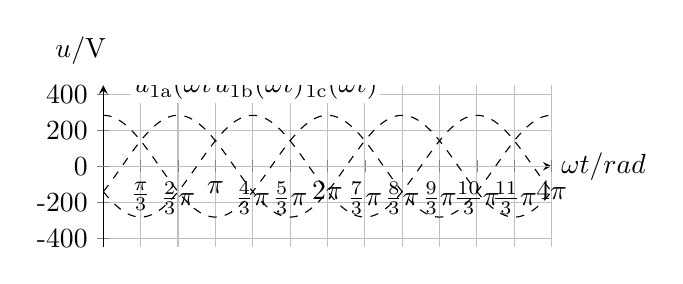
\begin{tikzpicture}
               \begin{axis}[
                   % x/y range adjustment
                   xmin=0, xmax=720,
                   ymin=-450, ymax=450,
                   samples=500,
                   axis y line=center,
                   axis x line=middle,
                   extra y ticks=0,
                   % Label text
                   xlabel={$\omega t / \text{rad}$},,
                   ylabel={$u/\mathrm{V}$},
                   % Label adjustment
                   x label style={at={(axis description cs:1,0.5)},anchor=west},
                   y label style={at={(axis description cs:-.05,.97)},anchor=south,yshift=0.2cm},
                   width=0.6\textwidth,
                   height=0.3\textwidth,
                   % x-Ticks
                   xtick={0,60,120,180,240,300,360, 420, 480, 540, 600, 660, 720},
                   xticklabels={,$\frac{\pi}{3}$,$\frac{2}{3}\pi$,$\pi$, $\frac{4}{3}\pi$,$\frac{5}{3}\pi$,$2\pi$, $\frac{7}{3}\pi$, $\frac{8}{3}\pi$,$\frac{9}{3}\pi$,$\frac{10}{3}\pi$,$\frac{11}{3}\pi$,$4\pi$},
                   xticklabel style = {anchor=north},
                   % y-Ticks
                   ytick={400,200,0,-200,-400},
                   yticklabels={400,200,0,-200,-400},
                   yticklabel style = {anchor=east},
                   % Grid layout
                   grid,
                   %grid style={line width=.1pt, draw=gray!10},
                   %major grid style={line width=.2pt,draw=gray!90},
                     ]
               % Voltage u1a(wt), u1b(wt) u1c(wt)
               \addplot[black, domain= 0:720,dashed] {282.84*cos(x)};
               \addplot[black, domain= 0:720,dashed] {282.84*cos(x+120)};
               \addplot[black, domain= 0:720,dashed] {282.84*cos(x+240)};
               % Label of u1c
               \node[black, fill=white, inner sep = 1pt, anchor = south] at (axis cs:370,350) {$u_{\mathrm{1c}}(\omega t)$}; 
               % Label of u1a
               \node[black, fill=white, inner sep = 1pt, anchor = south] at (axis cs:120,350) {$u_{\mathrm{1a}}(\omega t)$};           
               % Label of u1b
               \node[black, fill=white, inner sep = 1pt, anchor = south] at (axis cs:250,350) {$u_{\mathrm{1b}}(\omega t)$};

           \end{axis}     
           \end{tikzpicture}
           \caption{Output voltage $u_\mathrm{2}(t)$ for $\alpha$.}
           \label{fig:Task03_M3C_with_RLE}
   \end{figure}
\begin{solutionblock}
%%%%%%%%%%%%%%%%%%%%%%%%%%%%%%%%%%%%%%%%%%%%%%%%%%%%%%%%%%%%%%%%%%%%%%%%%%
% Output voltage u2 for M3C with RLE-Load
%%%%%%%%%%%%%%%%%%%%%%%%%%%%%%%%%%%%%%%%%%%%%%%%%%%%%%%%%%%%%%%%%%%%%%%%%%
\begin{solutionfigure}[htb]
    %   \documentclass{standalone}
    %   \usepackage{pgfplots}
    %   \pgfplotsset{compat=1.18} % Kompatibilität für neuere Versionen
           \centering
           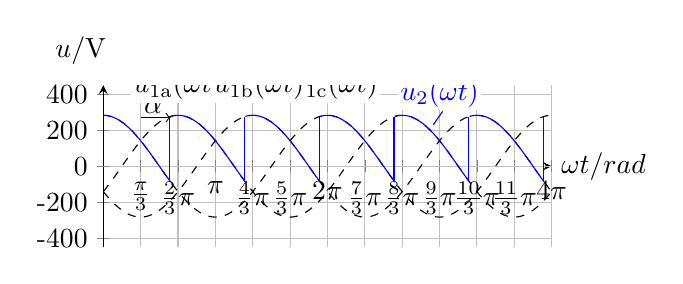
\begin{tikzpicture}
               \begin{axis}[
                   % x/y range adjustment
                   xmin=0, xmax=720,
                   ymin=-450, ymax=450,
                   samples=500,
                   axis y line=center,
                   axis x line=middle,
                   extra y ticks=0,
                   % Label text
                   xlabel={$\omega t / \text{rad}$},,
                   ylabel={$u/\mathrm{V}$},
                   % Label adjustment
                   x label style={at={(axis description cs:1,0.5)},anchor=west},
                   y label style={at={(axis description cs:-.05,.97)},anchor=south,yshift=0.2cm},
                   width=0.6\textwidth,
                   height=0.3\textwidth,
                   % x-Ticks
                   xtick={0,60,120,180,240,300,360, 420, 480, 540, 600, 660, 720},
                   xticklabels={,$\frac{\pi}{3}$,$\frac{2}{3}\pi$,$\pi$, $\frac{4}{3}\pi$,$\frac{5}{3}\pi$,$2\pi$, $\frac{7}{3}\pi$, $\frac{8}{3}\pi$,$\frac{9}{3}\pi$,$\frac{10}{3}\pi$,$\frac{11}{3}\pi$,$4\pi$},
                   xticklabel style = {anchor=north},
                   % y-Ticks
                   ytick={400,200,0,-200,-400},
                   yticklabels={400,200,0,-200,-400},
                   yticklabel style = {anchor=east},
                   % Grid layout
                   grid,
                   %grid style={line width=.1pt, draw=gray!10},
                   %major grid style={line width=.2pt,draw=gray!90},
                     ]
               % Voltage u1a(wt), u1b(wt) u1c(wt)
               \addplot[black, domain= 0:720,dashed] {282.84 *cos(x)};
               \addplot[black, domain= 0:720,dashed] {282.84 *cos(x+120)};
               \addplot[black, domain= 0:720,dashed] {282.84 *cos(x+240)};
   
               % Voltage u2(wt)
               \addplot[blue, domain= 0:108.17] {282.84 *cos(x)}; 
               \addplot[blue, domain= 108.17:228.17] {282.84 *cos(x+240)};     
               \addplot[blue, domain= 228.17:348.17] {282.84 *cos(x+120)};    
               \addplot[blue, domain= 348.17:468.17] {282.84 *cos(x)};
               \addplot[blue, domain= 468.17:588.17] {282.84 *cos(x+240)}; 
               \addplot[blue, domain= 588.17:708.17] {282.84 *cos(x+120)};
               \addplot[color=blue,solid] coordinates{
                (106.84,-81.94)   %(60+alpha,282.84*cos(60+alpha))
                (106.84, 275.41) %(60+alpha,282.84*cos(60+alpha + 240))
                };               
               \addplot[color=blue,solid] coordinates{
                   (226.84,-81.94)
                   (226.84, 275.41)
                };     
               \addplot[color=blue,solid] coordinates{
                   (346.84,-81.94)
                   (346.84,  275.41)
                };     
               \addplot[color=blue,solid] coordinates{
                   (466.84,-81.94)
                   (466.84, 275.41)
                };
               \addplot[color=blue,solid] coordinates{
                (586.84,-81.94)
                (586.84, 275.41)
                };               
               \addplot[color=blue,solid] coordinates{
                   (706.84,-81.94)
                   (706.84, 275.41)
                };     
                % Label of u2
               \node[blue, fill=white, inner sep = 1pt, anchor = south] at (axis cs:540,310) {$u_{\mathrm{2}}(\omega t)$};
                % Line to u2
               \draw[thin, blue] (545,305) -- (530,230);
                %Label alpha
               \node[black, fill=white, inner sep = 1pt, anchor = south] at (axis cs:80,275){$\alpha$};
               % Line for alpha
               \draw[->](60,270) -- (108.17,270);
           
               % Label of u1c
               \node[black, fill=white, inner sep = 1pt, anchor = south] at (axis cs:370,350) {$u_{\mathrm{1c}}(\omega t)$}; 
               % Label of u1a
               \node[black, fill=white, inner sep = 1pt, anchor = south] at (axis cs:120,350) {$u_{\mathrm{1a}}(\omega t)$};           
               % Label of u1b
               \node[black, fill=white, inner sep = 1pt, anchor = south] at (axis cs:250,350) {$u_{\mathrm{1b}}(\omega t)$};

           \end{axis}     
           \end{tikzpicture}
           \caption{Output voltage $u_\mathrm{2}(t)$ for $\alpha = 46.84$.}
           \label{sfig:subtask3.1_output_voltage}
   \end{solutionfigure}
\end{solutionblock}
\subtask{For the same $\alpha$, calculate the average output voltage $\bar{u}_\mathrm{2}$.}{2}
\subtaskGerman{ Berechnen Sie für dasselbe $\alpha$ die mittlere Ausgangsspannung $\bar{u}_\mathrm{2}$}
\begin{solutionblock}
Recalling the average output voltage equation in CCM:
$$\bar{u}_\mathrm{2}(\alpha) = \frac{3\sqrt{3}}{2\pi}\hat{u}_\mathrm{1}\cos(\alpha),$$            
where the peak value $\hat{u}_\mathrm{1}$ can be calculated as:
$$ \hat{u}_\mathrm{1} = \sqrt{2}U_\mathrm{1}= \sqrt{2}\cdot\SI{230}{\volt} \approx \SI{325.27}{\volt}.$$
Hence, the average output voltage is:
$$ \bar{u}_\mathrm{2}(\alpha=\frac{\pi}{3}) = \frac{3\sqrt{3}}{2\pi}\cdot \SI{325.27}{\volt}\cdot\cos(\frac{\pi}{3}) \approx \SI{134.5}{\volt}.$$
\end{solutionblock}
\subtask{Calculate the corresponding average load current $I_\mathrm{2}$.}{1}
\subtaskGerman{Berechnen Sie den entsprechenden mittleren Laststrom $I_2$.}
\begin{solutionblock}
The average output voltage can be written as:
$$ \bar{u}_\mathrm{2}(\alpha) = I_\mathrm{2}R + U_\mathrm{batt}.$$
Accordingly, the average output current can be calculated as:
$$  I_\mathrm{2} =  \frac{\bar{u}_\mathrm{2}(\alpha) - U_\mathrm{batt}}{R}=  \frac{\SI{134.5}{\volt} - \SI{125}{\volt}}{\SI{0.1}{\Omega}} = \SI{95}{\ampere}.$$
\end{solutionblock}
\subtask{Calculate the power loss in the resistor and the power delivered to the battery $U_\mathrm{batt}$.}{2}
\subtaskGerman{Berechnen Sie die an die Batterie $U_\mathrm{batt}$ abgegebene Leistung und die Verluste im Widerstand.}
\begin{solutionblock}
The power dissipated by the resistor can be calculated by:
            $$ P_\mathrm{resistor} = I^2_\mathrm{2} \cdot R = (\SI{95}{\ampere})^2 \cdot \SI{0.1}{\Omega} = \SI{902.5}{\watt},$$
            or using the voltage across the resistor by:
           $$ P_\mathrm{resistor} = (\bar{u}_\mathrm{2}(\alpha=\frac{\pi}{3}) - U_\mathrm{batt})\cdot I_\mathrm{2} = (\SI{134.5}{\volt} - \SI{125}{\volt}) \cdot \SI{95}{\ampere} = \SI{902.5}{\watt},$$
while the power delivered to $U_\mathrm{batt}$ is:
           $$ P_\mathrm{batt} =U_\mathrm{batt}\cdot I_\mathrm{2} = \SI{125}{\volt} \cdot \SI{95}{\ampere} = \SI{11.875}{\kilo\watt}.$$
\end{solutionblock}
\subtask{Consider the case where the inductance $L$ is finite, such that the converter operates in DCM. For an output voltage $u_\mathrm{2}$ where $\alpha = \frac{\pi}{3}$ and $\beta = \frac{\pi}{2}$, as shown in \autoref{fig:M3C_dcm}, calculate the average output voltage $\bar{u}_\mathrm{2}$.}{3}
\begin{hintblock}
In this question, the DCM is directly influenced by the presence of the battery voltage, which is different from having a capacitive filter at the output.
\end{hintblock}
\subtaskGerman{Betrachten Sie den Fall, dass die Induktivität $L$ nun nur noch endlich groß ist, so dass der Wandler im Lückebetrieb arbeitet,
wie in \autoref{fig:M3C_dcm} dargestellt. Für $\alpha = \frac{\pi}{3}$ und $\beta = \frac{\pi}{2}$ ist die mittlere Ausgangsspannung zu berechnen.}
\begin{germanhintblock}
In dieser Frage wird der DCM direkt von der Batteriespannung beeinflusst, was sich von einem kapazitiven Filter am Ausgang unterscheidet.
\end{germanhintblock}

\begin{figure}[htb]
        \begin{tikzpicture} % M1C output voltage
            \tikzmath{
                    real \Lw, \u1, \b, \adcm, \E, \R;
                    \Lw = 2; %angular frequency times inductance
                    \u1 = 1; %Input voltage amplitude
                    \b = 0.5*pi; %conduction interval for DCM
                    \adcm = pi/3; %firing angle for DCM (\b + \adcm must be greater than 2pi/3 for correct visualization)
                    \Ebatt= 0.4; %battery voltage
                    \R = 0.1;
                }
            \begin{groupplot}[group style={group size= 1 by 1, xticklabels at = edge bottom, vertical sep=1em, yticklabels at = edge left, horizontal sep = 1em}, 
                width=1\textwidth,
                height=0.34\textheight,
                axis x line=bottom,
                axis y line=left,
                xmin=0, xmax=4*pi,
                ymin=-1.15, ymax=1.15,
                xtick={0, pi/2, pi, 3*pi/2, 2*pi, 5*pi/2, 3*pi, 7*pi/2, 4*pi},
                xticklabels={$0$,$\frac{1}{2}\pi$, $\pi$,$\frac{3}{2}\pi$, $2\pi$,$\frac{5}{2}\pi$, $3\pi$, $\frac{7}{2}\pi$, $4\pi$},
                ytick={-1, -1/2, 0,1/2, 1},
                yticklabels={$-\hat{u}_\mathrm{s}$, ,$0$, ,$\hat{u}_\mathrm{2}$},
                grid=both,
                clip=false
                ]

            \nextgroupplot[title=DCM, height=0.35\textheight] % voltage DCM
                %\addplot[domain=0:4*pi, samples=200, signalblue, thick, name path = A3]{(x < \b) * cos(deg(x)) + (x > \adcm + pi/3)*(\adcm + pi/3 + \b > x)* cos(deg(x+(4*pi/3)))  + (x > \adcm + pi)*( \adcm + pi + \b > x)*cos(deg(x+(2*pi/3)))+ (x > 5*pi/3 + \adcm)* (x < 5*pi/3 + \adcm+ \b) * cos(deg(x)) + (x > \adcm + 7*pi/3)*(\adcm + (7*pi/3) + \b > x)* cos(deg(x+(4*pi/3)))+ (x > \adcm + 3*pi)*( \adcm + (3*pi) + \b > x)*cos(deg(x+(2*pi/3)))};
                
                \addplot[domain=0:4*pi, samples=200, signalblue, thick, name path = A3]{(x < pi/3 + \adcm +\b - 2*pi/3) * cos(deg(x)) + (x > pi/3 +\adcm + \b - 2*pi/3) * (x < pi/3 +\adcm) * \Ebatt+ (x > pi/3+\adcm)* (x < pi/3+\adcm + \b) * cos(deg(x+(4*pi/3)))+ (x > pi/3 + \adcm + \b) * (x < pi + \adcm ) * \Ebatt+ (x > \adcm + pi)*( \adcm + pi + \b > x) *cos(deg(x+(2*pi/3))) + (\adcm + pi + \b < x)* (x < 5*pi/3 + \adcm) * \Ebatt+ (x > 5*pi/3 +\adcm) * (x < 5*pi/3 + \adcm + \b) * cos(deg(x))+(x > 5*pi/3 + \adcm + \b)*(x < 7*pi/3 + \adcm) *\Ebatt + (x > 7*pi/3 + \adcm) *  (x < 7*pi/3 + \adcm + \b)*cos(deg(x+(4*pi/3))) + (x > 7*pi/3 + \adcm + \b)*(x < 3*pi + \adcm) *\Ebatt+ (x > 3*pi + \adcm) *  (x < 3*pi + \adcm + \b)*cos(deg(x+(2*pi/3))) + (x > 3*pi + \adcm + \b)*\Ebatt};
                  
               
                %\addplot[domain=0:4*pi, samples=10, signalblue, thick,dashed, name path = avg3]{\ucdcm};
                \addplot[domain=0:4*pi, samples=10, signalblue, thick,dashed, name path = avg3]{\Ebatt};
               % \node at (axis cs:-0.3,\ucdcm) [anchor=north] {$\overline{u}_2$};
                \node at (axis cs:-0.3,\Ebatt) [anchor=north] {$U_\mathrm{batt}$};
                \addplot[domain=0:4*pi, samples=50, signalgreen, dashed]{cos(deg(x))};
                \addplot[domain=0:4*pi, samples=50, signalbrown, dashed]{cos(deg(x+(2*pi/3)))};
                \addplot[domain=0:4*pi, samples=50, signalyellow, dashed]{cos(deg(x+(4*pi/3)))};
                \node at (axis cs:pi/3,-0.85) [signalbrown, fill=white,inner sep=1pt] {$u_\mathrm{1b}$};
                \node at (axis cs:pi,-0.85) [signalgreen, fill=white,inner sep=1pt] {$u_\mathrm{1c}$};
                \node at (axis cs:pi*6.7/4,-0.85) [signalyellow, fill=white,inner sep=1pt] {$u_\mathrm{1a}$};
                \draw[->] (axis cs:pi/3,1) -- node[above]{$\alpha$} (axis cs:pi/3+\adcm,1) ;
                \draw[->] (axis cs:pi,1) -- node[above]{$\alpha$} (axis cs:pi+\adcm,1) ;
                 \draw[->] (axis cs:5*pi/3,1) -- node[above]{$\alpha$} (axis cs:5*pi/3+\adcm,1) ;
                \draw[->] (axis cs:7*pi/3,1) -- node[above]{$\alpha$} (axis cs:7*pi/3+\adcm,1) ;
                 \draw[->] (axis cs:3*pi,1) -- node[above]{$\alpha$} (axis cs:3*pi+\adcm,1);
                 \draw[->] (axis cs:11*pi/3,1) -- node[above]{$\alpha$} (axis cs:11*pi/3+\adcm,1) ;
                \draw[dashed, thick] (axis cs:pi/3,0) -- (axis cs:pi/3,1);
                \draw[dashed, thick] (axis cs:pi,0) -- (axis cs:pi,1);
                 \draw[dashed, thick] (axis cs:5*pi/3,0) -- (axis cs:5*pi/3,1);
                \draw[dashed, thick] (axis cs:7*pi/3,0) -- (axis cs:7*pi/3,1);
                \draw[dashed, thick] (axis cs:3*pi,0) -- (axis cs:3*pi,1);
                 \draw[dashed, thick] (axis cs:11*pi/3,0) -- (axis cs:11*pi/3,1);
                \addplot[shadecolor, opacity=0.3] fill between[of=A3 and avg3, soft clip={domain=0:4*pi}];
                \draw[<->, thick] (axis cs:pi/3 +\adcm,-0.5) -- node[above]{$\beta$} (axis cs:pi/3 +\adcm + \b,-0.5) ;
            %    \draw[dashed, thick] (axis cs:pi/3 + \adcm,\E) -- (axis cs:pi/3 + \adcm,-0.5);
            %    \draw[dashed, thick] (axis cs:pi/3 + \adcm + \b,\E) -- (axis cs:pi/3 + \adcm + \b,-0.5);
           
            \end{groupplot}
        \end{tikzpicture}   
        \caption{M3C voltages in DCM.}
        \label{fig:M3C_dcm}
    \end{figure}
\begin{solutionblock}
In DCM mode, the inductor's current falls below the thyristors holding current, resulting in all thyristors stop conducting during certain intervals within the cycle. Since the output voltage during the non-conducting intervals is $u_\mathrm{2}(t) = U_\mathrm{batt}$, the average output voltage can be calculated as:

            $$\bar{u}_\mathrm{2}(\beta) = \frac{3}{2\pi} \left[\int_{0}^{\beta} \hat{u}_\mathrm{1}\cos(\omega t) \mathrm{d}\omega t +  \int_{\beta}^{\frac{2\pi}{3}} U_\mathrm{batt} \mathrm{d}\omega t \right].$$
            After integration, we get
           $$  \bar{u}_\mathrm{2}(\beta) = \frac{3}{2\pi} \left[ \hat{u}_\mathrm{1}(\sin(\beta)-\sin(0))  + U_\mathrm{batt} (\frac{2\pi}{3} - \beta)\right].$$
            So, for the given $\beta =\frac{\pi}{2}$, the average output voltage is
           $$  \bar{u}_\mathrm{2}(\beta) = \frac{3}{2\pi} \left[ \SI{325.27}{\volt}\cdot(\sin(\frac{\pi}{2})-\sin(0))  + \SI{125}{\volt} \cdot (\frac{2\pi}{3} - \frac{\pi}{2})\right] \approx \SI{186.55}{\volt}.$$

\end{solutionblock}